\section*{Схема экспериментальной установки}

Схема экспериментальной установки изображена на рисунке:

\begin{figure}[H]
	\centering
	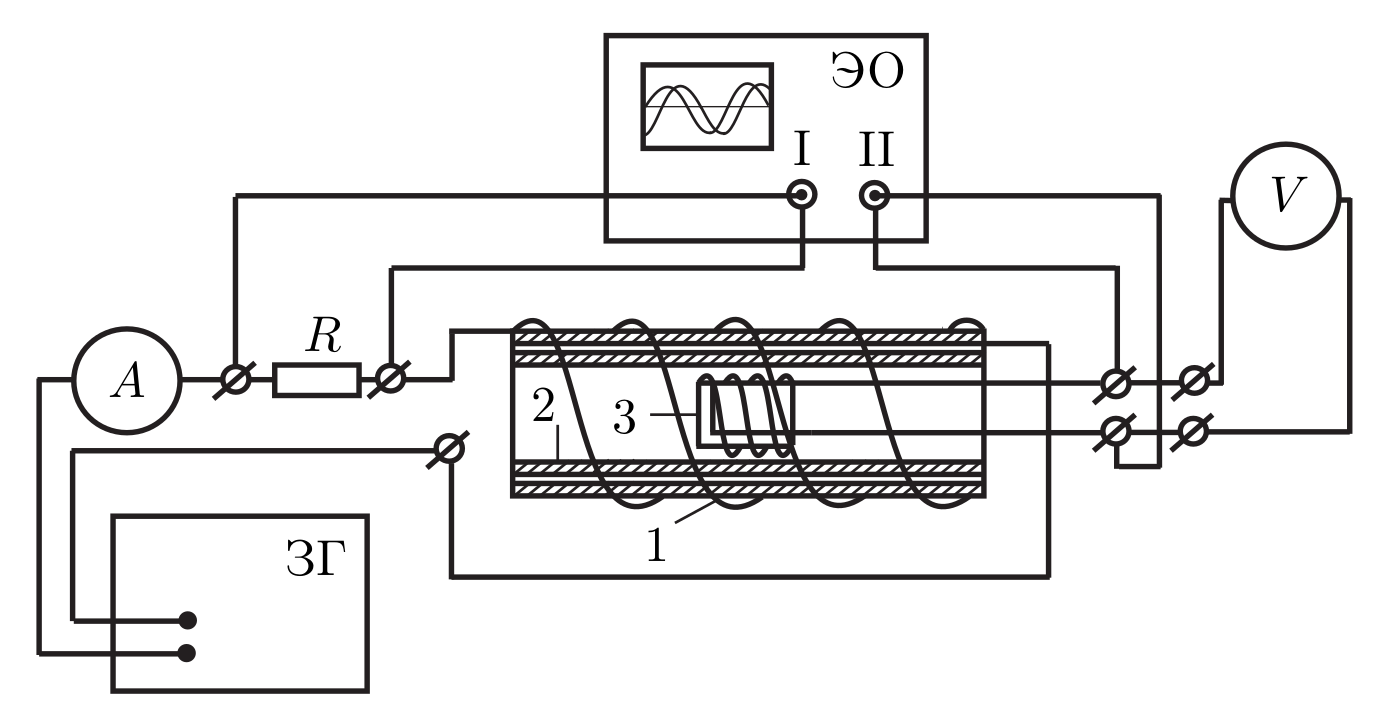
\includegraphics[width=0.7\textwidth]{../res/exp scheme.png}
\end{figure}

Переменное магнитное поле создаётся соленоидом, подключенным к генератору звуковой частоты ЗГ. Соленоид намотан на полый цилиндрический каркас из поливинилхлорида 1, в который вставлен медный цилиндр 2. Для измерения магнитного поля внутри цилиндра используется измерительная катушка 3. Действующие значения тока и напряжения в цепи измеряются соответственно амперметром $A$ и вольтметром $V$. Для измерения сдвига фаз используется осциллограф ЭО. Один вход осциллографа подключен к резистору, напряжение на котором пропорционально току в цепи. Второй вход подключен к измерительной катушке.

ЭДС индукции, возникающая в измерительной катушке равна
$$
U = - SN \frac{dB_1(t)}{dt} = -i \omega \mu_0 SN H_1 e^{i\omega t}
$$
Действующее значение напряжения, измеряемое вольтметром
$$
U = \frac{SN \omega}{\sqrt{2}} \mu_0 |H_1|
$$
Магнитное поле внутри цилиндра пропорционально напряжению и обратно пропорционально частоте:
$$
|H_1| \propto \frac{U}{\nu}
$$
Магнитное поле снаружи катушки пропорционально пропускаемому току:
$$
|H_0| \propto I
$$
Тогда 
$$
\frac{|H_1|}{|H_0|} = C \cdot \frac{U}{\nu I}
$$
где $C$ -- некоторая константа. Эта константа может быть экспериментально измерена при малых частотах, так как при $\nu \rightarrow 0$, выполняется $\frac{|H_1|}{|H_0|} \rightarrow 1$.

Так как материал, из которого изготовлен цилиндр может содержать примеси, то в работе измеряется проводимость данного цилиндра. Для этого измеряется зависимость сдвига фаз между $H_1$ и $H_0$ в области больших частот, строится зависимость $\varphi(\sqrt{\omega})$ по формуле (\ref{formula:delta_phi}) и по углу наклона прямой определяется проводимость материала.